% ============================================================================
%  EEE3095S CS Project 2026: Serial Game Server
%  STUDENT REPORT TEMPLATE (IEEE conference format, max 10 pages incl. refs)
% ============================================================================
%
%  How to use this template
%  ------------------------
%  * Red text in [square brackets] is PLACEHOLDER text. Replace every piece of
%    it with your own words. Search the PDF for "[" before you submit.
%  * Grey boxes are GUIDANCE. They tell you what the marker looks for. Leave
%    them on while you write, then switch them off below (\guidancefalse) to
%    check your length against the 10-page limit and before you submit.
%  * Dashed boxes are PLACEHOLDER FIGURES. Replace each with your own diagram
%    (\includegraphics{figures/yourfile.pdf} or TikZ).
%  * Keep the section headings exactly as they are: they are the brief's
%    required headings, in the brief's order, and the marking guide follows
%    them. Add your own subsection headings underneath.
%  * Build:  latexmk -pdf main.tex   (or upload the folder to Overleaf).
% ============================================================================
\documentclass[conference]{IEEEtran}

\usepackage[T1]{fontenc}
\usepackage{cite}
\usepackage{amsmath}
\usepackage{graphicx}
\usepackage{booktabs}
\usepackage{array}
\usepackage{xcolor}
\usepackage{listings}
\usepackage{tikz}
\usetikzlibrary{arrows.meta,positioning,calc,shapes.geometric}
\usepackage[most]{tcolorbox}
\usepackage[hidelinks]{hyperref}

% ---------------------------------------------------------------- switches --
\newif\ifguidance
\guidancetrue        % <-- change to \guidancefalse to hide all guidance boxes

% ------------------------------------------------------- template helpers --
\definecolor{phred}{rgb}{0.75,0.08,0.08}
\definecolor{guidebg}{gray}{0.94}
\definecolor{guideframe}{gray}{0.55}

% Placeholder text: replace with your own.
\newcommand{\ph}[1]{\textcolor{phred}{[#1]}}

% Guidance box: what the marker expects. Hidden when \guidancefalse.
\newtcolorbox{guidebox}[1][]{
  breakable, enhanced, colback=guidebg, colframe=guideframe,
  boxrule=0.4pt, arc=1pt, left=3pt, right=3pt, top=2pt, bottom=2pt,
  fontupper=\footnotesize\sffamily, title={#1},
  fonttitle=\footnotesize\sffamily\bfseries, coltitle=black,
  colbacktitle=guidebg!80!gray, before skip=4pt, after skip=6pt}
\newenvironment{guidance}[1][Guidance]
  {\ifguidance\begin{guidebox}[#1]\else\setbox0\vbox\bgroup\fi}
  {\ifguidance\end{guidebox}\else\egroup\fi}

% Placeholder figure: dashed box with a description of what to draw.
% Usage: \figph{<height>}{<what the figure must show>}
\newcommand{\figph}[2]{%
  \begin{tikzpicture}
    \draw[dashed, phred, line width=0.6pt] (0.3pt,0) rectangle (\linewidth-0.3pt,#1);
    \node[text width=0.85\linewidth, align=center, text=phred, font=\footnotesize]
      at (0.5\linewidth,0.5*#1) {#2};
  \end{tikzpicture}}

% allow line breaks after underscores (long test names in tables)
\renewcommand{\_}{\textunderscore\penalty0\hskip0pt\relax}
\newcolumntype{L}[1]{>{\raggedright\arraybackslash}p{#1}}

\lstset{
  basicstyle=\ttfamily\scriptsize, columns=fullflexible, keepspaces=true,
  frame=tb, framerule=0.4pt, commentstyle=\color{gray}\itshape,
  keywordstyle=\bfseries, showstringspaces=false, breaklines=true,
  captionpos=b, float=tp, floatplacement=tp,
}
\renewcommand{\lstlistingname}{Listing}

\begin{document}

% ---------------------------------------------------------------- title ----
\title{An Authoritative STM32F051 Tic-Tac-Toe Server\\with a Thin Python Client\\[2pt]
\normalsize Line-framed ASCII protocol, server-side validation and an automated board test suite}

\author{
\IEEEauthorblockN{Sibongokuhle Sibiya (\ph{student number})\quad
                  \ph{Student B full name} (\ph{student number})}
\IEEEauthorblockA{EEE3095S CS Project 2026, Department of Electrical Engineering\\
University of Cape Town}
}

\maketitle

\begin{abstract}
We built a two-player Tic-Tac-Toe server on an STM32F051 board that acts as the
only referee, and a Python/Tkinter client that forwards clicks and draws what
the server confirms. The two sides talk over the board's ST-Link virtual COM
port (USART1, 115200~baud, 8N1) using newline-terminated ASCII frames of at
most 63 characters. The server checks every request in a fixed order before it
writes any state, so a rejected request leaves the game unchanged. It answers
malformed, oversized, non-printable and incomplete frames with specific
\texttt{NACK} codes. We added three optional extensions: a CRC-8 frame
checksum, an AI opponent that moves through the same function as a human, and
move history with undo. A pytest harness drives the real board without human
input: 23 core tests and 24 extension tests. On the first run on the board,
21 of the 23 core tests passed (the extension tests did not exist yet). The two
failures exposed UART overruns in the HAL receive path, which we replaced with
a register-level interrupt handler. \ph{Final result: N of 47 tests pass on the
board after the fix; add the number once you have re-run the suite.}
\end{abstract}

\begin{guidance}[Before you start writing]
\begin{itemize}\setlength\itemsep{0pt}
\item \textbf{Marks} (brief, p.~6): Introduction 10, Protocol 15, Specification
  and design 15, Implementation 15, Game logic and server authority 15,
  Robustness 10, Validation 15, Conclusion 5. Video and Code links are required.
\item \textbf{Limit:} 10 pages \emph{including} references. Switch guidance off
  (\texttt{\textbackslash guidancefalse} in \texttt{main.tex}) to see your true length.
\item \textbf{Write headings that state a finding}, not just a topic, e.g.
  ``Validation runs before any state change'' rather than ``Validation''.
  Keep the section headings below as they are.
\item \textbf{Be specific}: name your mechanisms and give numbers
  (``rejects frames longer than 32 bytes''), not adjectives (``robust'',
  ``efficient'', ``significant'').
\item \textbf{Every figure, table and listing must be referred to and explained
  in the text.} Say what the reader should notice.
\item \textbf{Never present a result you did not measure.} If something is still
  untested on the board, say so.
\end{itemize}
\end{guidance}

\section{Introduction}
\label{sec:intro}

\begin{guidance}[Introduction (10 marks), about half a page]
The marker wants: the context and goal of the project; your \textbf{selected
game} and \textbf{GUI library}, with the reason for each choice; your main
\textbf{design choices}; the \textbf{task allocation} between the two of you; and
the \textbf{structure} of the report. Keep it to about half a page (brief,
p.~6). Open with the problem, not with the technology. Expand every acronym at
first use, e.g.\ ``finite-state machine (FSM)''.
\end{guidance}

A serial game has two programs that can disagree about the state of the game.
If the PC is trusted, a faulty or hostile client can place two marks in one
turn, overwrite an occupied cell or keep playing after the game has ended, and
the board and the screen then show different games. The project brief~\cite{brief}
therefore makes the STM32 the referee. My design guarantees one property: a
request that the server rejects never changes the game state.

I chose Tic-Tac-Toe, the baseline game in the brief, so that my effort went
into the protocol, the robustness of the server and the automated tests rather
than into game rules. % CONFIRM: reword if you had a different reason.
The client uses Tkinter~\cite{tkinter} because it ships with the standard
Python installer and needs no extra installation, and pySerial~\cite{pyserial}
for the serial port. % CONFIRM: reword if you had a different reason.

Beyond the compulsory system I built three of the optional extensions that
the brief lists or recommends: a CRC-8 checksum on every frame, an AI opponent,
and move history with undo. Each one sits behind new commands, so the compulsory
protocol behaves exactly as before and the 23 core tests still apply.

Three design choices shape the system. First, the firmware splits reception in
two: a short interrupt handler stores each byte in a ring buffer, and the main
loop assembles lines, parses them and runs the state machine. Second, the
protocol is line-framed ASCII with no spaces, so a person can test the server
from a serial terminal. Third, one pytest harness drives the real board
without human interaction, and every robustness rule has a named test.

\textbf{Task allocation and plan.} The brief allows teams of two; I worked alone,
so I did all of the work: protocol, firmware, GUI, test harness, extensions and
this report. Table~\ref{tab:plan} lists the milestones in the order I worked.

\begin{table}[t]
\centering
\caption{Project plan: milestones and outputs.}
\label{tab:plan}
\footnotesize
\begin{tabular}{@{}L{0.3cm}L{4.9cm}L{2.2cm}@{}}
\toprule
 & Milestone and output & Date \\
\midrule
1 & Protocol and server FSM specified & 10/10/2026 \\
2 & Firmware: framing, state machine, validation & 16/10/2026 \\
3 & Tkinter GUI client & 16/10/2026 \\
4 & Test harness, 23 core tests; first board run & 16/10/2026 \\
5 & Receive-path fix after the failed tests & 24/10/2026 \\
6 & Extensions: checksum, AI, undo, 24 more tests & 24/10/2026 \\
7 & Final board runs, report, video, repository & 27/10/2026 \\
\bottomrule
\end{tabular}
\end{table}

\textbf{Structure.} Section~\ref{sec:protocol} defines the requirements, the
message protocol and the extensions. Section~\ref{sec:design} presents the server FSM, the GUI
flowchart and the circuit. Section~\ref{sec:impl} explains five code excerpts.
Section~\ref{sec:authority} argues that the server stays authoritative.
Section~\ref{sec:robust} covers framing and recovery from bad input.
Section~\ref{sec:valid} reports the tests on the board, and
Section~\ref{sec:conclusion} concludes.

\section{Requirements and Message Protocol}
\label{sec:protocol}

\begin{guidance}[Requirements and message protocol (15 marks)]
Describe and diagram your \textbf{final} protocol: physical link (interface,
baud rate, frame format), \textbf{framing} (terminator, maximum frame length,
timeout), \textbf{board encoding}, the complete \textbf{command set}, and
\textbf{every response and error}. Cover new game, move, win/draw and
disconnect. Include at least one \textbf{sequence diagram}. \textbf{Highlight
every departure} from the brief's reference protocol (p.~3) and justify each
one. A reader should be able to write a compatible client from this section
alone.
\end{guidance}

\subsection{Newline-terminated frames of at most 63 characters}
The link is USART1 on PA9 (TX) and PA10 (RX), routed through the on-board
ST-Link virtual COM port~\cite{schematic}: 115200 baud, 8 data bits, no
parity, 1 stop bit, no flow control. Table~\ref{tab:framing} lists the framing
rules. Every rule has one reply, so a client can tell why a frame was refused.

\begin{table}[t]
\centering
\caption{Framing rules and the response to each violation.}
\label{tab:framing}
\footnotesize
\begin{tabular}{@{}L{2.6cm}L{5.4cm}@{}}
\toprule
Rule & Server behaviour \\
\midrule
Terminator & \texttt{\textbackslash n} or \texttt{\textbackslash r} ends a frame; an empty frame is ignored, so \texttt{\textbackslash r\textbackslash n} gives one reply \\
Maximum length & 63 characters; the rest of the line is discarded up to the next terminator; one \texttt{NACK:TOOLONG} \\
Incomplete frame & no terminator for 500~ms after the last byte: frame discarded, \texttt{NACK:TIMEOUT} \\
Invalid character & any byte outside 0x20--0x7E: frame discarded, \texttt{NACK:BADCMD} \\
UART fault & overrun, framing or noise error, or a full 128-byte receive ring: frame discarded, \texttt{NACK:BADCMD} \\
Checksum & optional suffix \texttt{*HH} (CRC-8); a wrong value gives \texttt{NACK:CHECKSUM} and nothing runs \\
\bottomrule
\end{tabular}
\end{table}

\subsection{An optional CRC-8 suffix catches errors that still look like commands}
Any frame may end in \texttt{*HH}, two hex digits of a CRC-8 (polynomial 0x07,
initial value 0, no reflection) over everything before the asterisk; for example
\texttt{MOVE:4} becomes \texttt{MOVE:4*75}, and the standard check value is
\texttt{crc8("123456789")} $=$ \texttt{0xF4}. The server verifies a suffix
before it parses the command and sends \texttt{NACK:CHECKSUM} on a mismatch.
This catches a bit error that turns one valid command into another, such as
\texttt{MOVE:4} into \texttt{MOVE:5}, which the framing rules cannot see. A
reply carries a suffix exactly when the request did, so a client that sends
plain frames is unaffected. Text that only looks like a suffix, such as
\texttt{NEW*ZZ}, is not a checksum and is rejected as \texttt{NACK:BADCMD}.

\subsection{Nine characters encode the board}
The board is nine characters, cells 0 to 8 row by row, using \texttt{.} for
empty, \texttt{X} and \texttt{O}. For example, \texttt{XO.XO....} is X in cells
0 and 3, O in cells 1 and 4, and everything else empty. X always moves first.

\subsection{Nine requests and one unsolicited message}
Table~\ref{tab:commands} lists the command set. The client sends one request at
a time and waits for the reply. The only message the server sends on its own is
\texttt{OK:BOARD:.........}, which follows a new game started with the
board's button; the client treats it like the reply to \texttt{NEW}, so the
display stays in step with the board.

\begin{table}[t]
\centering
\caption{Command set. $^\dagger$ marks a departure from the brief.}
\label{tab:commands}
\scriptsize
\begin{tabular}{@{}L{1.9cm}L{1.8cm}L{4.3cm}@{}}
\toprule
Request & Accepted in & Success response \\
\midrule
\texttt{CONNECT} & any state$^\dagger$ & \texttt{OK} (opens the session) \\
\texttt{NEW} & IDLE, GAME\_OVER & \texttt{OK:BOARD:<9>} \\
\texttt{NEW:AI}$^\dagger$ & IDLE, GAME\_OVER & \texttt{OK:BOARD:<9>}; the AI plays O \\
\texttt{MOVE:<i>} & IN\_PROGRESS & \texttt{OK:BOARD:<9>}, \texttt{WIN:X}, \texttt{WIN:O} or \texttt{DRAW}; in AI mode the board after the AI's reply \\
\texttt{MOVE:<i>:<m>}$^\dagger$ & IN\_PROGRESS & as above; \texttt{<m>} is X or O \\
\texttt{STATE} & IN\_PROGRESS, GAME\_OVER & \texttt{BOARD:<9>} \\
\texttt{HISTORY}$^\dagger$ & IN\_PROGRESS, GAME\_OVER & \texttt{HIST:<i>,<i>,...} \\
\texttt{UNDO}$^\dagger$ & IN\_PROGRESS & \texttt{OK:BOARD:<9>} \\
\texttt{RESIGN} & IN\_PROGRESS & \texttt{OK:GAMEOVER} \\
\texttt{DISCONNECT} & any state$^\dagger$ & \texttt{OK} (returns to IDLE) \\
Button press$^\dagger$ & session open & unsolicited \texttt{OK:BOARD:.........} \\
\bottomrule
\end{tabular}
\end{table}

\subsection{Every failure has its own NACK and a fixed check order}
Table~\ref{tab:errors} lists every error. When a request could fail several
checks, the server uses one order: framing first, then whether the command is
known, then the session, then the game state, and for \texttt{MOVE} the index
syntax, the index range, the turn and the cell. A checksum, if present, is
checked right after framing. Each request therefore has
exactly one correct reply.

\begin{table}[t]
\centering
\caption{Every error response and when the server sends it.}
\label{tab:errors}
\footnotesize
\begin{tabular}{@{}L{2.5cm}L{5.5cm}@{}}
\toprule
Response & Sent when \\
\midrule
\texttt{NACK:BADCMD} & unknown or wrong-case command, bad \texttt{MOVE} syntax, non-printable byte, UART fault, or \texttt{NEW} during a game \\
\texttt{NACK:NOGAME} & \texttt{MOVE}, \texttt{STATE} or \texttt{RESIGN} with no live game (IDLE, or \texttt{MOVE}/\texttt{RESIGN} after game over) \\
\texttt{NACK:RANGE} & index is negative or above 8 \\
\texttt{NACK:OCCUPIED} & the cell already holds a mark \\
\texttt{NACK:NOTURN}$^\dagger$ & the optional mark is not the side to move \\
\texttt{NACK:NOCONN}$^\dagger$ & a known command arrives before \texttt{CONNECT} \\
\texttt{NACK:TOOLONG}$^\dagger$ & frame longer than 63 characters \\
\texttt{NACK:TIMEOUT}$^\dagger$ & frame not terminated within 500~ms \\
\texttt{NACK:CHECKSUM}$^\dagger$ & the \texttt{*HH} suffix does not match the payload \\
\texttt{NACK:NOUNDO}$^\dagger$ & \texttt{UNDO} with no move to take back \\
\bottomrule
\end{tabular}
\end{table}

\subsection{Departures from the reference protocol}
\textbf{Optional mark on \texttt{MOVE}.} With one client playing both sides,
the server cannot see an out-of-turn move in \texttt{MOVE:<i>}. The suffix
\texttt{:<m>} names the player; the server answers \texttt{NACK:NOTURN} if
\texttt{<m>} is not the side to move, which makes the rule testable. The GUI
does not send the suffix. \textbf{\texttt{CONNECT} and \texttt{DISCONNECT} in
any state.} A reconnecting client works after a crash, and closing the GUI
mid-game always returns the server to IDLE. \textbf{Extra errors.}
\texttt{NOCONN}, \texttt{TOOLONG} and \texttt{TIMEOUT} give a specific reply
to a specific fault instead of one generic error. \textbf{Unsolicited board.}
The button needs a way to tell the client that a new game began.
\textbf{Extensions.} The checksum suffix, \texttt{NEW:AI}, \texttt{HISTORY},
\texttt{UNDO} and their replies are optional additions; none of them changes the
reply to a compulsory request.

\begin{figure}[t]
\centering
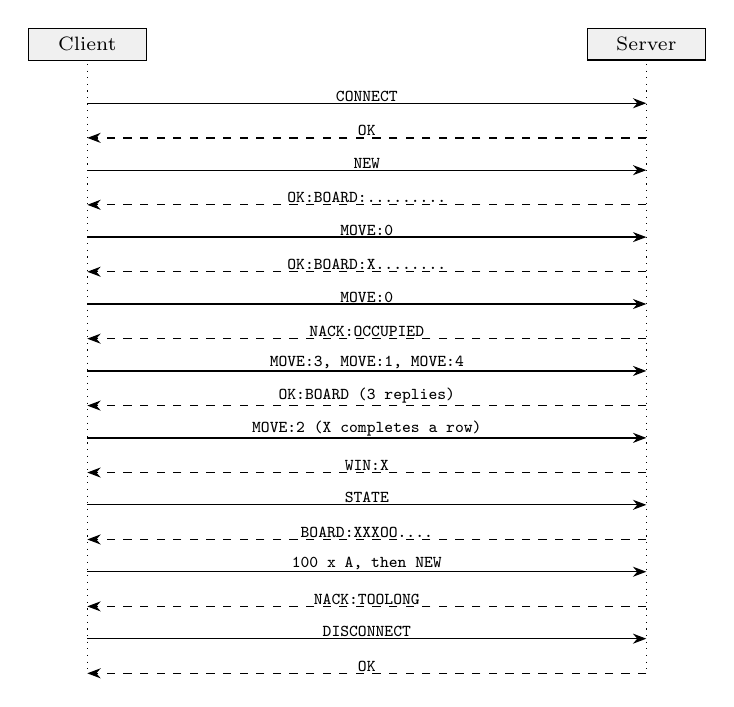
\begin{tikzpicture}[font=\scriptsize,
  msg/.style={-{Stealth[length=1.7mm]},line width=0.45pt},
  rep/.style={-{Stealth[length=1.7mm]},line width=0.45pt,dashed},
  lab/.style={above,pos=0.5,inner sep=0.5pt,font=\fontsize{6.3}{7}\selectfont}]
  \node[draw,fill=gray!12,minimum width=1.5cm] (c) at (0.8,0) {Client};
  \node[draw,fill=gray!12,minimum width=1.5cm] (s) at (7.9,0) {Server};
  \draw[dotted] (0.8,-0.25) -- (0.8,-8.0);
  \draw[dotted] (7.9,-0.25) -- (7.9,-8.0);
  \foreach \y/\req/\rsp in {
     1/{CONNECT}/{OK},
     2/{NEW}/{OK:BOARD:.........},
     3/{MOVE:0}/{OK:BOARD:X........},
     4/{MOVE:0}/{NACK:OCCUPIED},
     5/{MOVE:3, MOVE:1, MOVE:4}/{OK:BOARD (3 replies)},
     6/{MOVE:2 (X completes a row)}/{WIN:X},
     7/{STATE}/{BOARD:XXXOO....},
     8/{100 x A, then NEW}/{NACK:TOOLONG},
     9/{DISCONNECT}/{OK}} {
    \draw[msg] (0.8,{-0.85*\y+0.1}) -- node[lab]{\texttt{\req}} (7.9,{-0.85*\y+0.1});
    \draw[rep] (7.9,{-0.85*\y-0.34}) -- node[lab]{\texttt{\rsp}} (0.8,{-0.85*\y-0.34});
  }
\end{tikzpicture}

\caption{One session. A rejected move (step 4) is answered with a NACK and
the game continues; a win (step 6) ends the game; an oversized line (step 8) is
refused without running the \texttt{NEW} at its end. Replies are dashed.}
\label{fig:sequence}
\end{figure}

Figure~\ref{fig:sequence} shows one session. After the second \texttt{MOVE:0}
is refused with \texttt{NACK:OCCUPIED}, the game continues from the same
board. After the win, \texttt{STATE} returns the final board, because the
server sends only \texttt{WIN:X} and not the board. In step 8 the server
discards the whole 103-character line, including the \texttt{NEW} at its end.

\section{Specification and Design}
\label{sec:design}

\begin{guidance}[Specification and design (15 marks)]
Required (brief, A.3--A.5): an \textbf{embedded server FSM} covering IDLE,
IN\_PROGRESS, GAME\_OVER \textbf{and the move-validation branch}; a
\textbf{flowchart of the GUI application}; and a \textbf{circuit diagram} of the
STM-to-PC UART connection, with the on-board button and LED behaviour labelled.
Diagrams may be at function level. Explain \textbf{why} responsibilities sit on
the server or the client. Draw diagrams in a tool that exports vector PDF
(draw.io, TikZ, Mermaid) and check that every label is readable when printed.
\end{guidance}

\subsection{The server decides; the client only draws}
Table~\ref{tab:owner} assigns each decision to one side. The server holds the
only copy of the game state (the board, the side to move and the game status)
and the client never computes any of it. The firmware has two layers. Hardware
code covers the USART interrupt, polled transmit, the LED and the button.
Rule code covers \texttt{check\_win}, \texttt{check\_draw},
\texttt{handle\_move} and the command dispatcher, which depend only on the
game variables and on \texttt{send\_str}. I kept the rules apart from the
interrupt and LED code so that they never depend on timing.

\begin{table}[t]
\centering
\caption{Who owns each decision.}
\label{tab:owner}
\footnotesize
\begin{tabular}{@{}L{3.5cm}L{1.3cm}L{3.0cm}@{}}
\toprule
Decision & Owner & Why \\
\midrule
Board, turn, game status & server & one source of truth \\
Is a move legal? & server & a client cannot be trusted \\
Win and draw detection & server & result must match the LED \\
Session (\texttt{CONNECT}) & server & rejects commands before it \\
What is drawn & client & only from \texttt{OK:BOARD}, \texttt{BOARD} \\
AI move choice & server & same write path as a human \\
Move history, undo & server & client keeps no move list \\
LED and button & server & board-side indicators \\
\bottomrule
\end{tabular}
\end{table}

\subsection{Three states and a validation chain that writes last}
Figure~\ref{fig:fsm} shows the server FSM. In IDLE the server accepts
\texttt{NEW} (or \texttt{NEW:AI}) once a session is open. In IN\_PROGRESS it accepts
\texttt{MOVE}, \texttt{STATE}, \texttt{HISTORY}, \texttt{UNDO} and \texttt{RESIGN}; a legal
move stays in IN\_PROGRESS unless it wins or fills the board. In GAME\_OVER it accepts
\texttt{NEW}, \texttt{STATE} and \texttt{HISTORY}, and a \texttt{MOVE} or \texttt{UNDO} gets
\texttt{NACK:NOGAME}. \texttt{DISCONNECT} returns any
state to IDLE. The lower part of the figure expands the validation branch. The
five checks come before the first write to the board, so every
\texttt{NACK} exit leaves the state unchanged. The figure omits the
\texttt{NOCONN}, \texttt{TOOLONG}, \texttt{TIMEOUT} and \texttt{CHECKSUM} replies, which belong
to the framer and the session check and never reach the state machine.

\begin{figure*}[t]
\centering
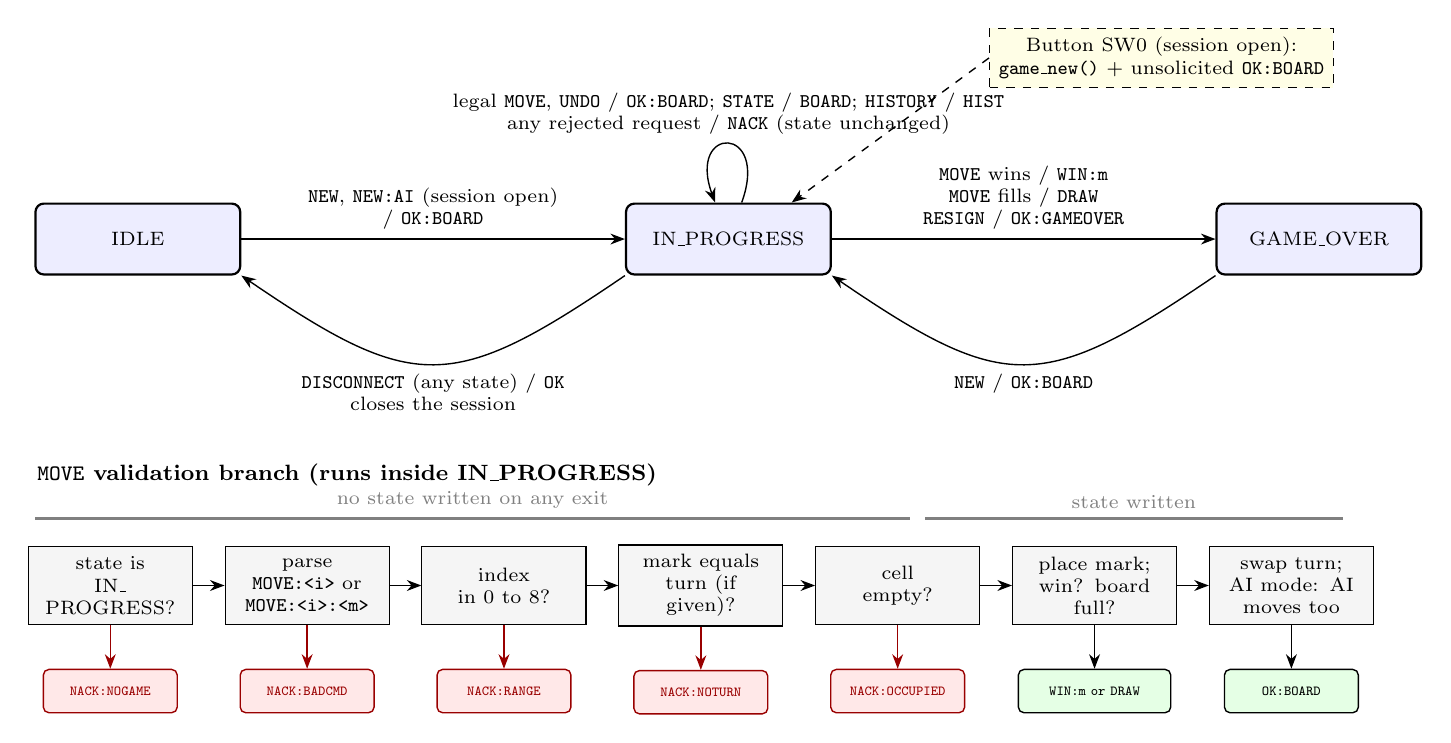
\begin{tikzpicture}[font=\scriptsize,>=Stealth,
  st/.style={draw,rounded corners=3pt,minimum width=2.6cm,minimum height=0.9cm,fill=blue!7,thick},
  bx/.style={draw,minimum width=1.95cm,minimum height=1.0cm,text width=1.85cm,align=center,fill=gray!8},
  nk/.style={draw,rounded corners=2pt,fill=red!9,font=\tiny\ttfamily,minimum width=1.7cm,minimum height=0.55cm,align=center},
  ok/.style={draw,rounded corners=2pt,fill=green!10,font=\tiny\ttfamily,minimum width=1.7cm,minimum height=0.55cm,align=center},
  ar/.style={->,line width=0.5pt}]
  % ---- states
  \node[st] (idle) at (1.6,0) {IDLE};
  \node[st] (prog) at (9.1,0) {IN\_PROGRESS};
  \node[st] (over) at (16.6,0) {GAME\_OVER};
  \draw[ar] (idle.east) -- node[above,align=center]{\texttt{NEW}, \texttt{NEW:AI} (session open)\\ / \texttt{OK:BOARD}} (prog.west);
  \draw[ar] (prog.east) -- node[above,align=center]{\texttt{MOVE} wins / \texttt{WIN:m}\\\texttt{MOVE} fills / \texttt{DRAW}\\\texttt{RESIGN} / \texttt{OK:GAMEOVER}} (over.west);
  \draw[ar] (prog.70) to[out=70,in=110,looseness=8]
     node[above,align=center]{legal \texttt{MOVE}, \texttt{UNDO} / \texttt{OK:BOARD}; \texttt{STATE} / \texttt{BOARD}; \texttt{HISTORY} / \texttt{HIST}\\any rejected request / \texttt{NACK} (state unchanged)} (prog.110);
  \draw[ar] (over.south west) .. controls +(-2.2,-1.5) and +(2.2,-1.5) .. node[below,pos=0.5]{\texttt{NEW} / \texttt{OK:BOARD}} (prog.south east);
  \draw[ar] (prog.south west) .. controls +(-2.2,-1.5) and +(2.2,-1.5) .. node[below,pos=0.5,align=center]{\texttt{DISCONNECT} (any state) / \texttt{OK}\\closes the session} (idle.south east);
  \node[draw,dashed,align=center,fill=yellow!10] (btn) at (14.6,2.3) {Button SW0 (session open):\\\texttt{game\_new()} + unsolicited \texttt{OK:BOARD}};
  \draw[ar,dashed] (btn.west) -- (prog.30);
  % ---- validation chain
  \node[font=\footnotesize\bfseries,anchor=west] at (0.2,-3.0) {\texttt{MOVE} validation branch (runs inside IN\_PROGRESS)};
  \foreach \i/\t in {0/{state is\\IN\_PROGRESS?},1/{parse\\\texttt{MOVE:<i>} or\\\texttt{MOVE:<i>:<m>}},2/{index\\in 0 to 8?},3/{mark equals\\turn (if given)?},4/{cell\\empty?},5/{place mark;\\win? board full?},6/{swap turn;\\AI mode: AI\\moves too}} {
    \node[bx] (b\i) at ({1.25+2.5*\i},-4.4) {\t};
  }
  \foreach \i/\j in {0/1,1/2,2/3,3/4,4/5,5/6} {\draw[ar] (b\i) -- (b\j);}
  \foreach \i/\t in {0/NACK:NOGAME,1/NACK:BADCMD,2/NACK:RANGE,3/NACK:NOTURN,4/NACK:OCCUPIED} {
    \draw[ar,red!60!black] (b\i.south) -- ++(0,-0.55) node[nk,anchor=north] {\t};
  }
  \draw[ar] (b5.south) -- ++(0,-0.55) node[ok,anchor=north,font=\tiny\ttfamily,text width=1.7cm] {WIN:m or DRAW};
  \draw[ar] (b6.south) -- ++(0,-0.55) node[ok,anchor=north] {OK:BOARD};
  \draw[thick,gray] (0.3,-3.55) -- node[above]{no state written on any exit} (11.4,-3.55);
  \draw[thick,gray] (11.6,-3.55) -- node[above]{state written} (16.9,-3.55);
\end{tikzpicture}

\caption{Server FSM with the move-validation branch. Red exits are NACKs
that leave the state unchanged; green exits are successes. The symbol
\texttt{m} stands for the mark of the side to move.}
\label{fig:fsm}
\end{figure*}

\subsection{The GUI never blocks and never guesses}
Figure~\ref{fig:gui} shows the client flow. A reader thread blocks on the port and
puts each line into a queue; the Tk main loop empties the queue every 50~ms, so the
window stays responsive. After the port opens, the client resends
\texttt{CONNECT} every 600~ms, up to 15 times, so it works whether or not
opening the port reset the board. It keeps one request in flight and ignores
board clicks until the reply arrives or 2~s pass. It redraws the board only from
\texttt{OK:BOARD} or \texttt{BOARD}. After \texttt{WIN} or \texttt{DRAW} it
sends \texttt{STATE} and redraws from the answer. Every request carries a checksum;
the client ignores a reply with a wrong one and asks for \texttt{STATE} instead of
acting on it. A tick box chooses \texttt{NEW:AI}, and the Undo and History buttons send
one request each and show the server's answer, because the client keeps no move list. If the cable is unplugged,
the reader thread ends and the next request times out with ``No reply from
board''; a failed write sets the status line to the error.

\begin{figure}[t]
\centering
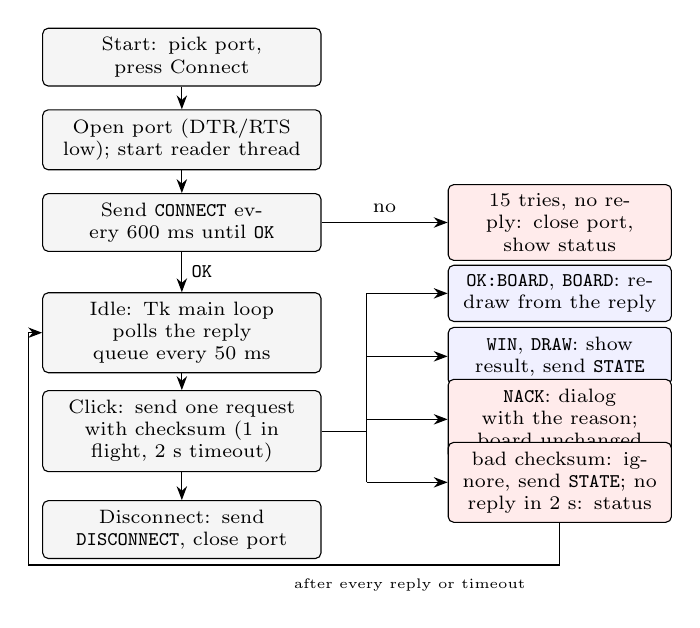
\begin{tikzpicture}[font=\scriptsize,>=Stealth,
  pr/.style={draw,rounded corners=2pt,fill=gray!8,text width=3.3cm,align=center,minimum height=0.62cm},
  rs/.style={draw,rounded corners=2pt,fill=blue!6,text width=2.6cm,align=center,minimum height=0.55cm},
  er/.style={draw,rounded corners=2pt,fill=red!8,text width=2.6cm,align=center,minimum height=0.55cm},
  ar/.style={->,line width=0.45pt}]
  \node[pr] (a) at (2.1,0)     {Start: pick port, press Connect};
  \node[pr] (b) at (2.1,-1.05) {Open port (DTR/RTS low); start reader thread};
  \node[pr] (c) at (2.1,-2.1)  {Send \texttt{CONNECT} every 600~ms until \texttt{OK}};
  \node[er] (cf) at (6.9,-2.1) {15 tries, no reply: close port, show status};
  \node[pr] (d) at (2.1,-3.5)  {Idle: Tk main loop polls the reply queue every 50~ms};
  \node[pr] (e) at (2.1,-4.75) {Click: send one request with checksum (1 in flight, 2~s timeout)};
  \node[pr] (g) at (2.1,-6.0)  {Disconnect: send \texttt{DISCONNECT}, close port};
  \node[rs] (r1) at (6.9,-3.0)  {\texttt{OK:BOARD}, \texttt{BOARD}: redraw from the reply};
  \node[rs] (r2) at (6.9,-3.8)  {\texttt{WIN}, \texttt{DRAW}: show result, send \texttt{STATE}};
  \node[er] (r3) at (6.9,-4.6)  {\texttt{NACK}: dialog with the reason; board unchanged};
  \node[er] (r4) at (6.9,-5.4)  {bad checksum: ignore, send \texttt{STATE}; no reply in 2~s: status};
  \draw[ar] (a) -- (b); \draw[ar] (b) -- (c);
  \draw[ar] (c.east) -- node[above]{no} (cf.west);
  \draw[ar] (c) -- node[right]{\texttt{OK}} (d);
  \draw[ar] (d) -- (e); \draw[ar] (e) -- (g);
  % one request, four possible outcomes
  \draw (e.east) -- (4.45,-4.75) -- (4.45,-3.0);
  \foreach \r/\y in {r1/-3.0,r2/-3.8,r3/-4.6,r4/-5.4} {
    \draw[ar] (4.45,\y) -- (\r.west);
  }
  \draw (4.45,-5.4) -- (4.45,-4.75);
  % every outcome returns to the idle loop
  \draw[ar] (r4.south) -- (6.9,-6.45) -- (0.15,-6.45) -- (0.15,-3.5) -- (d.west);
  \node[font=\tiny,anchor=north west] at (3.4,-6.5) {after every reply or timeout};
\end{tikzpicture}

\caption{GUI application flowchart. Every board change comes from a reply
line, never from the click itself.}
\label{fig:gui}
\end{figure}

\subsection{One USB cable carries power, programming and the serial link}
Figure~\ref{fig:circuit} shows the circuit. USART1 TX (PA9) and RX (PA10)
connect to the ST-Link's virtual COM port on the board, so no extra wiring or
USB-UART converter is used, and the two share ground through the board. The
dual-colour LED D9 sits on PB10 (red) and PB11 (green) behind 150\,$\Omega$
resistors and lights when the pin is high. Red means X to move, green means O
to move, both blinking means game over, and both off means IDLE. Button SW0 on
PA0 reads low when pressed (the firmware enables the internal pull-up) and
starts a new game if a session is open. On my board the red and green dies
are physically swapped, so one constant (\texttt{BOARD\_RG\_SWAPPED}) swaps the
two pins in software.

\begin{figure}[t]
\centering
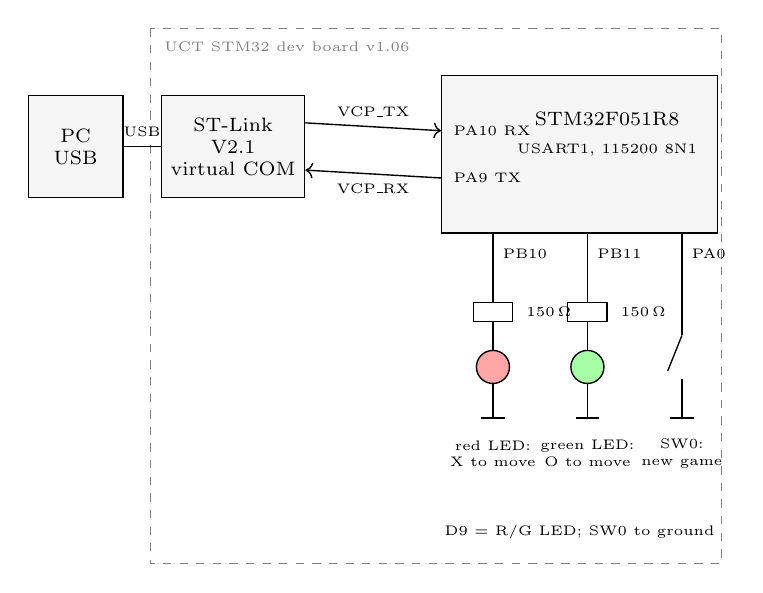
\begin{tikzpicture}[font=\scriptsize,line width=0.5pt,
  box/.style={draw,align=center,fill=gray!8},
  res/.style={draw,minimum width=0.5cm,minimum height=0.24cm,fill=white,inner sep=0pt}]
  \draw[dashed,gray] (1.55,1.5) rectangle (8.8,-5.3);
  \node[anchor=north west,font=\tiny,gray] at (1.6,1.45) {UCT STM32 dev board v1.06};
  \node[box,minimum width=1.2cm,minimum height=1.3cm] (pc) at (0.6,0) {PC\\USB};
  \node[box,minimum width=1.6cm,minimum height=1.3cm] (stl) at (2.6,0) {ST-Link\\V2.1\\virtual COM};
  \node[box,minimum width=3.5cm,minimum height=2.0cm] (mcu) at (7.0,-0.1) {};
  \node at (7.35,0.35) {STM32F051R8};
  \node[font=\tiny] at (7.35,-0.05) {USART1, 115200 8N1};
  \draw (pc.east) -- node[above,font=\tiny]{USB} (stl.west);
  \draw[->] ([yshift=0.3cm]stl.east) -- node[above,font=\tiny]{VCP\_TX} ([yshift=0.3cm]mcu.west);
  \draw[<-] ([yshift=-0.3cm]stl.east) -- node[below,font=\tiny]{VCP\_RX} ([yshift=-0.3cm]mcu.west);
  \node[font=\tiny,anchor=west] at ([xshift=1pt,yshift=0.3cm]mcu.west) {PA10 RX};
  \node[font=\tiny,anchor=west] at ([xshift=1pt,yshift=-0.3cm]mcu.west) {PA9 TX};
  % LED and button
  \foreach \x/\pin in {5.9/PB10,7.1/PB11,8.3/PA0} {
    \draw (\x,-1.1) -- (\x,-1.9);
    \node[font=\tiny,anchor=south west] at (\x,-1.55) {\pin};
  }
  \foreach \x/\col/\cap in {5.9/red/{red LED:\\X to move},7.1/green/{green LED:\\O to move}} {
    \node[res] at (\x,-2.1) {};
    \draw (\x,-1.9) -- (\x,-1.97); \draw (\x,-2.23) -- (\x,-2.6);
    \node[draw,circle,minimum size=0.42cm,inner sep=0pt,fill=\col!35] at (\x,-2.8) {};
    \draw (\x,-3.01) -- (\x,-3.45);
    \draw (\x-0.15,-3.45) -- (\x+0.15,-3.45);
    \node[font=\tiny,align=center] at (\x,-3.9) {\cap};
  }
  \node[font=\tiny,anchor=west] at (6.2,-2.1) {150\,$\Omega$};
  \node[font=\tiny,anchor=west] at (7.4,-2.1) {150\,$\Omega$};
  % button to ground
  \draw (8.3,-1.9) -- (8.3,-2.4); \draw (8.3,-2.4) -- (8.12,-2.85); \draw (8.3,-2.95) -- (8.3,-3.45);
  \draw (8.15,-3.45) -- (8.45,-3.45);
  \node[font=\tiny,align=center] at (8.3,-3.9) {SW0:\\new game};
  \node[font=\tiny] at (7.0,-4.9) {D9 = R/G LED; SW0 to ground};
\end{tikzpicture}

\caption{Circuit: UART link to the PC, the LED and the button.}
\label{fig:circuit}
\end{figure}

\section{Implementation}
\label{sec:impl}

\begin{guidance}[Implementation (15 marks)]
Choose \textbf{3 to 5 short code excerpts} that were \textbf{not straightforward}
to write, and explain each: what problem it solves, why you wrote it this way,
and what would go wrong with the obvious alternative. Good candidates:
receiving bytes in an interrupt and handing them to the main loop; the frame
assembler with timeout and oversize handling; non-blocking button debounce;
keeping the GUI responsive; separating unsolicited messages from replies.
Keep each listing short (10--25 lines) and narrow enough for one column; trim
comments and boilerplate, and say that you did. Do not paste whole files.
\end{guidance}

The listings in this report are trimmed: I removed comments, blank lines and
unrelated declarations.

\subsection{A register-level interrupt keeps up with 115200 baud}
Listing~\ref{lst:isr} is the receive path. At 115200 baud a byte arrives every
87\,$\mu$s. My first version re-armed \texttt{HAL\_UART\_Receive\_IT} after every
byte~\cite{um1785}. On the board it answered 6-character commands correctly,
but frames of 20 and 103 characters were answered with \texttt{NACK:BADCMD}
instead of \texttt{NACK:RANGE} and \texttt{NACK:TOOLONG}, which means the
server had flagged a UART fault mid-frame. I did not capture the overrun flag
directly, so overrun is my diagnosis from this evidence. The handler now reads
the status register and the data register itself~\cite{rm0091}, which is a few
dozen instructions long (I did not measure its run time). It clears the error flags, sets \texttt{rx\_fault}
so that the framer rejects the damaged frame, and pushes the byte into a
128-byte ring buffer. The interrupt only writes \texttt{rx\_head} and the main
loop only writes \texttt{rx\_tail}, so no lock is needed. The first version
also never enabled the USART1 interrupt in the NVIC, so no command arrived at
all; \texttt{HAL\_UART\_MspInit} now calls \texttt{HAL\_NVIC\_EnableIRQ}.

\begin{lstlisting}[float=tp, language=C, caption={Interrupt handler and ring buffer (\texttt{stm32f0xx\_it.c}, \texttt{main.c}).}, label=lst:isr]
void USART1_IRQHandler(void) {
    uint32_t isr = USART1->ISR;
    if (isr & (USART_ISR_ORE | USART_ISR_FE |
               USART_ISR_NE)) {
        USART1->ICR = USART_ICR_ORECF | USART_ICR_FECF
                    | USART_ICR_NCF;
        rx_fault = 1;               /* frame is damaged */
    }
    if (isr & USART_ISR_RXNE)
        uart_rx_push((uint8_t)USART1->RDR);
}
void uart_rx_push(uint8_t b) {
    uint16_t next = (rx_head + 1) % RX_RING_SIZE;
    if (next == rx_tail) rx_fault = 1;  /* ring full */
    else { rx_ring[rx_head] = b; rx_head = next; }
}
\end{lstlisting}

\subsection{The framer discards a bad line up to its terminator}
Listing~\ref{lst:framer} turns the byte stream into frames. The obvious
approach resets the buffer when a line is too long and carries on. Then the end
of a 100-character line would be parsed as a new command, so a line ending in
\texttt{NEW} would start a game. Instead the framer sets \texttt{frame\_err}
and drops every byte until the next terminator, then sends exactly one NACK.
A non-printable byte sets the same flag. A separate check in the main loop
compares \texttt{HAL\_GetTick()} with the time of the last received byte and
discards a half-received frame after 500~ms, so a lost terminator cannot glue
two commands together.

\begin{lstlisting}[float=tp, language=C, caption={Frame assembler (\texttt{main.c}).}, label=lst:framer]
while (rx_tail != rx_head) {
    char c = (char)rx_ring[rx_tail];
    rx_tail = (rx_tail + 1) % RX_RING_SIZE;
    last_rx_tick = HAL_GetTick();
    if (c == '\n' || c == '\r') {
        if (frame_err)
            send_str(frame_err == FE_TOOLONG
                ? "NACK:TOOLONG\n" : "NACK:BADCMD\n");
        else if (line_len > 0) {
            line_buf[line_len] = '\0';
            process_command(line_buf);
        }
        line_len = 0; frame_err = FE_NONE;
    } else if (frame_err) { /* drop until terminator */ }
    else if ((unsigned char)c < 0x20 ||
             (unsigned char)c > 0x7E)
        frame_err = FE_GARBAGE;
    else if (line_len < LINE_MAX_LEN)
        line_buf[line_len++] = c;
    else frame_err = FE_TOOLONG;
}
\end{lstlisting}

\subsection{The GUI waits on the port in a thread and draws from a queue}
Listing~\ref{lst:gui} shows how the client stays responsive (I split one line for width). A blocking
\texttt{readline} in a Tk callback would freeze the window for up to the
port timeout on every call. The worker thread is the only code that blocks on
the port; it hands lines to the Tk thread through a thread-safe queue, and the
Tk thread polls that queue every 50~ms and never blocks. The handshake uses
the same timer mechanism, so the GUI keeps sending \texttt{CONNECT} while the
board is still booting. Tkinter widgets are touched only from the Tk
thread~\cite{tkinter}.

\begin{lstlisting}[float=tp, language=Python, caption={Reader thread, queue polling and handshake (\texttt{gui\_client.py}).}, label=lst:gui]
def _read_thread(self, ser):       # worker thread
    while ser.is_open:
        raw = ser.readline()
        line = raw.decode(errors="replace").strip()
        if line:
            self.rx_queue.put(line)

def _poll_queue(self):             # Tk thread
    while not self.rx_queue.empty():
        self._handle_line(self.rx_queue.get())
    self.root.after(50, self._poll_queue)

def _handshake(self):              # until OK
    if not self.ser or self.connected: return
    if self.handshake_tries >= 15:
        self._close_port(); return
    self.handshake_tries += 1
    self._send("CONNECT")
    self.root.after(600, self._handshake)
\end{lstlisting}

\subsection{The AI searches a copy of the board and moves through the human's write path}
Listing~\ref{lst:ai} is the opponent's search: negamax with alpha-beta pruning,
scoring a win as $10-\mathit{depth}$ so that the AI prefers the quickest win and
the slowest loss. Two choices matter. First, the search places and removes marks
on a local copy of the board, so the game board changes only in
\texttt{apply\_move}, the single function that writes a mark; the human's
\texttt{MOVE} and the AI's reply both call it after their own checks, and the AI
re-checks that its chosen cell is empty first. A search that wrote to the real board
could leave a half-explored position behind. Second, cells are tried centre,
corners, then edges, which cuts the search: on a PC build of the same source the
worst single decision, the first reply, takes 1\,260 calls to \texttt{negamax}
(mean 35), against up to $8! = 40\,320$ move sequences without pruning. I have
not timed the search on the board, but in all five full test runs every AI reply
arrived inside the harness's 2~s read timeout. The search runs in the main loop
while the receive interrupt keeps buffering bytes.

\begin{lstlisting}[float=tp, language=C, caption={AI search (\texttt{main.c}, trimmed).}, label=lst:ai]
int negamax(char *b, char me, char opp,
            int depth, int alpha, int beta) {
    int best = -100;
    for (int k = 0; k < 9; k++) {
        int i = ai_order[k], sc;   /* 4,0,2,6,8,1,3,5,7 */
        if (b[i] != '.') continue;
        b[i] = me;
        if (line_win(b, me))    sc = 10 - depth;
        else if (board_full(b)) sc = 0;
        else sc = -negamax(b, opp, me, depth + 1,
                           -beta, -alpha);
        b[i] = '.';
        if (sc > best)     best = sc;
        if (best > alpha)  alpha = best;
        if (alpha >= beta) break;
    }
    return best;
}
\end{lstlisting}

\section{Game Logic and Server Authority}
\label{sec:authority}

\begin{guidance}[Game logic and server authority (15 marks)]
Show: correct \textbf{move validation}; rejection of \textbf{illegal,
out-of-turn and out-of-state} moves with specific errors; reliable
\textbf{win and draw detection}; and a \textbf{client-untrusted} design. Most
importantly, give an argument that a \textbf{rejected request cannot change the
server state}, based on how your code is structured (e.g. every check runs
before the first write), and point to the tests that check it. The brief calls
this a ``proof''; make it a step-by-step argument a reader can verify against
your code.
\end{guidance}

\subsection{Every check returns before the first write}
Listing~\ref{lst:move} is \texttt{handle\_move}. It runs the checks in the
order of Section~\ref{sec:protocol}: game state, syntax, range, turn, cell. Each
failing check sends one NACK and returns. The parser uses only local variables,
and saturates the number at 1000 so that a long digit string cannot overflow;
an earlier version used \texttt{atoi}, which turned \texttt{MOVE:abc} into a
move on cell 0.

\begin{lstlisting}[float=tp, language=C, caption={Move validation (\texttt{main.c}, trimmed).}, label=lst:move]
void handle_move(const char *p) {
    if (game_state != STATE_IN_PROGRESS)
        { send_str("NACK:NOGAME\n"); return; }
    int neg = 0, nd = 0, idx = 0; char mark = 0;
    if (*p == '-') { neg = 1; p++; }
    while (*p >= '0' && *p <= '9') {
        if (idx < 1000) idx = idx*10 + (*p - '0');
        p++; nd++;
    }
    if (nd == 0) { send_str("NACK:BADCMD\n"); return; }
    if (*p == ':') {
        mark = p[1];
        if ((mark != 'X' && mark != 'O') || p[2] != '\0')
            { send_str("NACK:BADCMD\n"); return; }
    } else if (*p != '\0')
        { send_str("NACK:BADCMD\n"); return; }
    if (neg || idx > 8)
        { send_str("NACK:RANGE\n"); return; }
    if (mark && mark != turn)
        { send_str("NACK:NOTURN\n"); return; }
    if (board[idx] != '.')
        { send_str("NACK:OCCUPIED\n"); return; }
    int r = apply_move(idx);  /* first write to the board */
    if (r == MV_CONTINUE && ai_mode) r = ai_reply();
    send_move_result(r);      /* WIN, DRAW or OK:BOARD */
}
\end{lstlisting}

\subsection{A rejected request cannot change the game state}
The game state is six variables: \texttt{board}, \texttt{turn},
\texttt{game\_state}, \texttt{connected}, \texttt{ai\_mode} and the move history.
The argument has five steps, and each step can be checked against \texttt{main.c}.
\begin{enumerate}\setlength\itemsep{0pt}
\item Only seven pieces of code write those variables: \texttt{game\_new()},
  \texttt{apply\_move()}, \texttt{handle\_undo()}, and the \texttt{CONNECT},
  \texttt{DISCONNECT}, \texttt{NEW} and \texttt{RESIGN} branches of
  \texttt{process\_command}. Every other path calls only \texttt{send\_str}.
\item \emph{Framing and checksum errors.} \texttt{process\_rx} calls
  \texttt{process\_command} only for a complete frame with \texttt{frame\_err}
  equal to zero and a checksum that is absent or correct. The oversize, garbage,
  fault, timeout and \texttt{CHECKSUM} branches send one NACK and reset
  \texttt{line\_len} and \texttt{frame\_err}, which belong to the framer, not to
  the game.
\item \emph{Unknown command or no session.} \texttt{process\_command} returns
  with \texttt{NACK:BADCMD} or \texttt{NACK:NOCONN} before it reaches any
  handler.
\item \emph{Handlers.} \texttt{NEW} returns with \texttt{NACK:BADCMD} before it
  sets \texttt{ai\_mode} or calls \texttt{game\_new()} when a game is running.
  \texttt{STATE} and \texttt{HISTORY} only read. \texttt{RESIGN} returns with
  \texttt{NACK:NOGAME} before it writes \texttt{game\_state}. \texttt{handle\_undo}
  checks the game state and the history length before it removes anything.
\item \emph{\texttt{MOVE}.} In Listing~\ref{lst:move} the call
  \texttt{apply\_move(idx)} is the first write, and every NACK path returns
  before it.
\end{enumerate}
Hence every path that ends in a NACK has written no game variable. This is an
argument from reading the code, not a formal proof, and the tests below sample
it. The button is not a request over the link: it is a local override that
resets the game when a session is open, and is documented as such.
\texttt{test\_occupied\_move\_rejected\_and\_board\_unchanged},
\texttt{test\_malformed\_move\_does\_not\_touch\_state},
\texttt{test\_new\_during\_game\_rejected\_state\_unchanged},
\texttt{test\_out\_of\_turn\_rejected},
\texttt{test\_wrong\_checksum\_rejected\_and\_nothing\_executed} and
\texttt{test\_undo\_all\_the\_way\_back\_then\_nothing\_to\_undo} each send a bad
request and then read \texttt{STATE} to compare the board. The oversize and
garbage tests check that a bad frame does not run the command at its end.

\subsection{The server alternates the turn and can check a named player}
The variable \texttt{turn} starts as X and flips only after a legal move that
neither wins nor draws. A plain \texttt{MOVE:<i>} is played by the side to move.
A \texttt{MOVE:<i>:<m>} with the wrong mark gets \texttt{NACK:NOTURN} before the
cell is examined, and \texttt{test\_out\_of\_turn\_rejected} checks that the board
is unchanged. In AI mode the human is always X, so a mark \texttt{O} on a
\texttt{MOVE} is also refused with \texttt{NACK:NOTURN}.

\subsection{The AI cannot make an illegal move}
\texttt{ai\_choose} considers only empty cells on a copy of the board, and
\texttt{ai\_reply} checks \texttt{board[idx] == '.'} again before it calls
\texttt{apply\_move}, the same function a human \texttt{MOVE} ends in. A legal AI
move is therefore true by construction, not by testing alone. Two checks back it
up. On a PC build of the same \texttt{main.c} I enumerated every possible human
strategy against the AI: 521 games, the human won none, the AI won 368 and 153
were draws.
\texttt{test\_ai\_never\_makes\_an\_illegal\_move\_and\_never\_loses} plays 20
seeded random games on the board and checks that each reply differs from the
previous board by exactly the human's X and one new O.

\subsection{Undo restores the board and the turn from the history}
The server stores the cell of every move. \texttt{UNDO} clears the last cell (the
last two in AI mode, so it is the human's turn again) and sets the turn from the
parity of the history length, so the turn can never disagree with the board. It
is refused after game over, because the result has already been sent, and with an
empty history it returns \texttt{NACK:NOUNDO}. \texttt{test\_undo\_restores\_board\_and\_turn}
and \texttt{test\_undo\_in\_ai\_mode\_removes\_both\_moves} check both modes.

\subsection{Win is checked before draw, for the mover only}
After placing a mark the server tests the eight lines (three rows, three columns,
two diagonals) for the mover's mark only, because only that mark can have just
completed a line. The win test runs before the draw test, so a ninth move that
completes a line is a win and not a draw. Either result sets
\texttt{GAME\_OVER}, after which \texttt{MOVE} returns \texttt{NACK:NOGAME}.
\texttt{test\_scripted\_win\_x}, \texttt{test\_scripted\_win\_o} and
\texttt{test\_scripted\_draw} cover these results. No test yet covers a win on the
ninth move, and Section~\ref{sec:conclusion} lists this as a limitation.

\subsection{The client holds no rules}
The GUI sends \texttt{MOVE:<i>} for any click, including a click on an occupied
cell, and shows the server's reason. If the client also checked legality, two
rule sets would have to stay identical, and they would disagree whenever the
button started a game that the client did not see. My own first GUI inferred
the final mark after a \texttt{WIN} from the move count. I removed that guess,
and the GUI now asks for \texttt{STATE}.

\section{Protocol Robustness and Integrity}
\label{sec:robust}

\begin{guidance}[Protocol robustness and integrity (10 marks)]
Show \textbf{framing}, \textbf{specific NACKs for malformed input}, and
\textbf{graceful recovery} from partial or garbage data. A table that maps each
kind of bad input to your mechanism, its response and the test that checks it
works well. Also explain why the server can never block forever (bounded
loops, timeouts, no blocking waits in the main loop). Give measured numbers
where you have them, e.g. the timeout you observed.
\end{guidance}

The server refuses every bad frame with a specific NACK, discards it up to the
next terminator or the 500~ms timeout, and answers the next valid command
normally. Table~\ref{tab:threats} maps each kind of bad input to the mechanism
and the test that exercises it.

\begin{table}[t]
\centering
\caption{Bad input, the server's handling, and the test that checks it.}
\label{tab:threats}
\scriptsize
\begin{tabular}{@{}L{1.55cm}L{3.0cm}L{3.45cm}@{}}
\toprule
Bad input & Handling and response & Test \\
\midrule
Partial frame & dropped after 500~ms of silence; \texttt{NACK:TIMEOUT} & \texttt{test\_partial\_frame\_times\_out\_and\_is\_discarded}; \texttt{test\_frame\_split\_across\_writes} (a split under 500~ms is reassembled) \\
Oversized frame & discarded to terminator; one \texttt{NACK:TOOLONG} & \texttt{test\_oversized\_frame\_rejected\_and\_tail\_not\_executed} \\
Garbage bytes & non-printable byte flags the frame; \texttt{NACK:BADCMD} & \texttt{test\_garbage\_bytes\_rejected\_then\_recovers} \\
Wrong case or unknown command & exact match only; \texttt{NACK:BADCMD} & \texttt{test\_unknown\_and\_wrong\_case\_commands}; \texttt{test\_malformed\_move\_does\_not\_touch\_state}; \texttt{test\_malformed\_suffix\_is\_not\_a\_checksum} \\
Corrupted bytes & CRC-8 suffix checked before parsing; \texttt{NACK:CHECKSUM}, nothing runs (frames that carry a suffix) & \texttt{test\_wrong\_checksum\_rejected\_and\_nothing\_executed}; \texttt{test\_corrupted\_payload\_is\_detected} \\
UART errors & flags cleared in the interrupt; frame rejected with \texttt{NACK:BADCMD} & no dedicated test; first seen through the oversize test \\
\bottomrule
\end{tabular}
\end{table}

\subsection{A 500 ms timeout is far longer than any frame}
A 64-byte frame takes about 5.6~ms on the wire (10 bits per byte at 115200
baud), so a healthy sender never reaches 500~ms between bytes, and a stalled
sender is cleared within about half a second. Our test checks only that the
\texttt{NACK:TIMEOUT} arrives inside the 2~s read window of the harness; we did
not measure the exact delay.

\subsection{The checksum detects corruption the framer cannot see}
Framing only checks the shape of a frame. A flipped bit that turns \texttt{MOVE:4}
into \texttt{MOVE:5} still has the right shape, so the framer accepts it and the
server would play the wrong cell. The CRC-8 suffix closes that gap for frames that
carry it: \texttt{test\_corrupted\_payload\_is\_detected} sends exactly that
substitution with the old checksum and checks that the board does not change. A CRC
with a degree-8 polynomial detects every single-bit error and every burst of up to
8 bits. The protection is optional: a plain frame has none, and damage to the
\texttt{*} or the two digits makes a checksummed frame look plain, when it is
usually (not provably) rejected as an unknown command.

\subsection{The next terminator resynchronises the stream}
A bad frame sets \texttt{frame\_err}, the framer drops the remaining bytes,
and the first \texttt{\textbackslash n} or \texttt{\textbackslash r} clears the flag
after one NACK. The tests send a bad frame and then a valid command, and
check that the valid command gets its normal reply and that the bad frame's
tail did not run (Listing~\ref{lst:framer}).

\subsection{No path in the main loop waits without a bound}
The framer loop ends when the ring is empty, which is at most 127 bytes. Transmit
is polled with a 100~ms timeout per message. The main loop contains no
\texttt{HAL\_Delay}: the button is debounced by comparing timestamps, and the only
delays are the three LED flashes (600~ms) at start-up, before any request is
accepted. We did not enable the independent watchdog, and
\texttt{Error\_Handler} halts only if the HAL initialisation itself fails.

\section{Validation}
\label{sec:valid}

\begin{guidance}[Validation and automated test harness (15 marks)]
Show \textbf{passing tests for every required case} and \textbf{screenshots or a
short video} of the working system. The brief's required tests (p.~4):
CONNECT returns OK and NEW returns an empty board; a legal move changes the
board exactly as expected; an occupied-cell move returns NACK:OCCUPIED and
leaves the board unchanged; an out-of-range move returns NACK:RANGE; a move
after game over returns NACK:NOGAME (or your documented equivalent); scripted
win and draw sequences return the correct result; and, if you built an AI
opponent, it never makes an illegal move. Map each one to a named test.
\textbf{Report results on the real board}, and say clearly which results come
from a simulator, if you used one.
\end{guidance}

\subsection{One fixture puts the board into a known state before every test}
The harness uses pytest~\cite{pytest} and pySerial~\cite{pyserial}. The port
name comes from the \texttt{SERIAL\_PORT} environment variable, and the suite
skips if it is unset, so it cannot fail on a machine without a board. Before each
test the fixture sends \texttt{CONNECT} until the board answers \texttt{OK}
(for up to 10~s, so it does not depend on the boot banner or on a reset when the
port opens), waits for stale replies, and sends \texttt{DISCONNECT}. Every test
therefore starts in IDLE with no session. Run the core suite with
\texttt{python -m pytest -v test\_protocol.py}, the extension suite with
\texttt{test\_extras.py}, and the whole suite with a checksum on every request by
setting \texttt{USE\_CRC=1}. The board results in this section come from the real
board on \texttt{COM14} (Windows, Python 3.11.9, pytest 7.4.3). Results from a PC
build of the firmware are labelled as such.

\subsection{21 of 23 tests passed on the first board run, and the two failures were real}
The core suite (\texttt{test\_protocol.py}) has 23 tests: the required cases of Table~\ref{tab:required}, the state
machine (\texttt{NOCONN}, \texttt{NOGAME}, \texttt{NOTURN}, resign, disconnect)
and the robustness cases of Table~\ref{tab:threats}. On the first run on the
board, 21 passed and 2 failed in 12.45~s; the extension tests did not exist yet. In \texttt{test\_out\_of\_range\_rejected}
the first four indices (9, 10, 99, $-1$) returned \texttt{NACK:RANGE}, but the
fifth, a 15-digit number, returned \texttt{NACK:BADCMD}. In the oversize test a
103-character line returned \texttt{NACK:BADCMD} instead of
\texttt{NACK:TOOLONG}. Both failures involve frames much longer than the
passing 6-character commands, which led us to the receive path described in
Section~\ref{sec:impl}. The second run, after we replaced the HAL receive path
with the register-level handler, is \ph{result: N passed, M failed in T s}.

\begin{table}[t]
\centering
\caption{The brief's required tests and their results on the board.}
\label{tab:required}
\scriptsize
\begin{tabular}{@{}L{3.2cm}L{3.0cm}cc@{}}
\toprule
Requirement (brief, p.~4) & Test name & Run 1 & Run 2 \\
\midrule
\texttt{CONNECT} returns \texttt{OK}; \texttt{NEW} returns an empty board & \texttt{test\_connect\_returns\_ok}; \texttt{test\_new\_returns\_empty\_board} & pass & \ph{res} \\
A legal move changes the board exactly as expected & \texttt{test\_legal\_move\_changes\_board\_exactly} & pass & \ph{res} \\
Occupied cell returns \texttt{NACK:OCCUPIED}, board unchanged & \texttt{test\_occupied\_move\_rejected\_and\_board\_unchanged} & pass & \ph{res} \\
Out-of-range move returns \texttt{NACK:RANGE} & \texttt{test\_out\_of\_range\_rejected} & fail & \ph{res} \\
Move after game over returns \texttt{NACK:NOGAME} & \texttt{test\_move\_after\_game\_over\_rejected} & pass & \ph{res} \\
Scripted win and draw give the correct result & \texttt{test\_scripted\_win\_x}; \texttt{test\_scripted\_win\_o}; \texttt{test\_scripted\_draw} & pass & \ph{res} \\
AI never makes an illegal move & \texttt{test\_ai\_never\_makes\_an\_illegal\_move\_and\_never\_loses} (\texttt{test\_extras.py}) & n/a & \ph{res} \\
\bottomrule
\end{tabular}
\end{table}

Table~\ref{tab:required} shows that the required behaviour was correct on the
first run except for very long indices. The out-of-range test failed only on its
last value; \texttt{NACK:RANGE} for 9, 10, 99 and $-1$ was already correct.

\subsection{24 extension tests check the checksum, the AI and undo}
Table~\ref{tab:ext} summarises \texttt{test\_extras.py}. The AI test plays 20 seeded
random games and checks that every reply differs from the previous board by
exactly the human's X and one new O, and that the human never wins. The checksum
tests include the substitution of \texttt{MOVE:4} by \texttt{MOVE:5} with the old
checksum, and the known CRC-8 value. Setting \texttt{USE\_CRC=1} reruns all 47
tests with a checksum on every request and verifies every reply.

\begin{table}[t]
\centering
\caption{Extension tests and their results on the board.}
\label{tab:ext}
\scriptsize
\begin{tabular}{@{}L{1.45cm}L{0.65cm}L{4.15cm}L{1.1cm}@{}}
\toprule
Group & Tests & What they check & Board \\
\midrule
Checksum & 9 & test vector, reply carries a suffix only if the request did, wrong checksum rejected, corrupted payload caught & \ph{res} \\
AI & 7 & one AI move per human move, blocks a threat, takes a win, 20 random games with no illegal AI move and no human win & \ph{res} \\
History, undo & 8 & move list, undo restores board and turn (both modes), \texttt{NOUNDO}, \texttt{NOGAME}, \texttt{NOCONN} & \ph{res} \\
All 47, \texttt{USE\_CRC=1} & 47 & the whole suite with a checksum on every request & \ph{res} \\
\bottomrule
\end{tabular}
\end{table}

\ph{Optional, keep only if you run the PC build (tools/hostsim) yourself: before flashing
we also ran all 47 tests against a PC build of \texttt{main.c} with the HAL stubbed out,
plain and with \texttt{USE\_CRC=1}, and all passed. This is not a board result.}

\begin{figure}[t]
\centering
\figph{5cm}{Screenshot of your GUI connected to the board, e.g. mid-game or
just after a rejected move, with the message the user sees.}
\caption{\ph{What the screenshot shows and what to notice in it.}}
\label{fig:screenshot}
\end{figure}

\ph{Refer to Fig.~\ref{fig:screenshot} here: one sentence on what the reader
should notice, e.g.\ the dialog for a rejected move.}

\subsection{Code review found five bugs before the board did, and the board found one more}
Reading the first firmware against the brief found five defects: the USART1
interrupt was never enabled, so no command was received; \texttt{atoi} turned
\texttt{MOVE:abc} into a move on cell 0; the tail of an oversized line ran as a
command; \texttt{NEW} was accepted in the middle of a game; and the hand-written
boards in the first draw test were wrong, so that test would have failed on
correct firmware. We fixed these before the first board run.
The board then exposed the receive-path overrun described in
Section~\ref{sec:impl}. \ph{Add any bug you hit while running the board or the GUI
that is not listed here.}

\section{Conclusion}
\label{sec:conclusion}

\begin{guidance}[Conclusion (5 marks)]
Summarise \textbf{success} (which requirements you met, with evidence),
\textbf{usefulness} (where this design would apply beyond the project),
\textbf{limitations} (be honest: what does not work, or only works under
conditions) and \textbf{possible improvements}. No new results here.
\end{guidance}

The server meets the compulsory requirements: it validates every request in a
fixed order before writing state, detects wins and draws, rejects illegal,
out-of-state and out-of-turn requests with specific NACKs, and recovers from
partial, oversized and garbage input. The evidence is the first board run, where
21 of 23 core tests passed, and \ph{the second run: N of 47}. The GUI connects,
plays, shows the server's rejection reasons and disconnects. The three optional
extensions work behind new commands: a CRC-8 checksum that stops a corrupted
but valid-looking command, an AI opponent that cannot make an illegal move, and
move history with undo.

\textbf{Usefulness.} The same pattern applies to any small device that must
accept commands from an untrusted host, such as a lab instrument or a motor
controller: a line-framed protocol with specific error codes, validation before
any state change, and a test harness that drives the real device.

\textbf{Limitations.} The checksum is optional, so a client that sends plain
frames has no protection, and a bit error in the suffix itself is not provably
caught. Undo works only while a game is in progress. One client plays both sides, so
\texttt{NACK:NOTURN} is exercised only through the optional mark that the GUI
does not send. The receive-path overrun is our diagnosis from test evidence, not
a captured flag. We measured no timing on the board: the 500~ms timeout is a
design value, and we did not time the AI's search there. We did not enable the watchdog. No test covers a win on the ninth
move. We ran everything on one board and one Windows PC, and the LED colours on
that board are swapped, which one constant corrects in software.

\textbf{Improvements.} A mandatory checksum mode would remove the unprotected
plain path. A second client (a second USART and a USB-UART adapter) would make
out-of-turn play real, and a hardware timer could add a move clock. The
independent watchdog would recover from a firmware fault.

\section{Video}
\label{sec:video}

\begin{guidance}[Video (required)]
A short video of \textbf{your group} demonstrating the working STM32 game
server: connect, legal moves, a rejected move, a win or draw, moves disabled
after game over, a new game, the button and LED behaviour, and disconnect.
Show the board and the screen. Check that the link works for someone who is
not logged in as you.
\end{guidance}

The demonstration video is available at \ph{link to video}.
\ph{One or two sentences on what the video shows, in order.}

\section{Code}
\label{sec:code}

\begin{guidance}[Code (required)]
Link to the GitHub repository with the STM32CubeIDE project, the GUI, the test
harness, and a README with setup, build, flash, run and test instructions.
Before you submit, clone it into a clean folder and follow your own README
(brief, p.~5). Make sure the repository is accessible to the markers.
\end{guidance}

The source code is at \ph{link to GitHub repository}. The repository holds the
STM32CubeIDE project (\texttt{Core/}, \texttt{Drivers/}, the \texttt{.ioc} file),
the Tkinter client (\texttt{python\_gui/}), the pytest harness (\texttt{tests/})
and a README with the directory tree and the build, flash, run and test steps.


\bibliographystyle{IEEEtran}
\bibliography{refs}

\end{document}
